\chapter{Implementatie}
Na de literatuurstudie en de ontwerpfase, is het tijd om het ontwerp dat besproken werd in Hoofdstuk~\vref{sec:anaEnOntwerp} te implementeren.
Als programmeertaal werd Python gekozen zodanig dat de applicatie uniform is met het testraamwerk.
In de komende secties worden de verschillende implementatie beslissingen toegelicht en wordt de geschreven code toegelicht.
De applicatie werd geschreven met twee doelen in het achterhoofd: de demo die gegeven gaat worden tijdens de verdediging en een basis vormen voor Televic om van te vertrekken.
Het doel van de presentatie is het tonen van het installatieproces beginnende bij de creatie van een installer tot het installeren zelf in een container in een field dock.
Om dit te kunnen realiseren, was het niet nodig/mogelijk om alle nodige functionaliteiten te implementeren en toe te voegen aan de applicatie.
Tijdens het implementeren, werden de server-side en client-side van elkaar gescheiden en er werden twee verschillende packages aangemaakt.
In wat volgt, zullen deze dan ook afzonderlijk besproken worden.

\section{Server-side}
\paragraph{Initialisatie} 
De server package bevat alle logica die hoort bij het release dock als bij de broker, maar bevat ook enkele modules die gebruikt worden om de realiteit af te beelden.
De flow van de applicatie begint met het opstarten van de deployment\_server module.
Deze module zal een release dock, een broker en een packager opstarten.
Vervolgens wordt het release dock gesubscribed voor de berichten van het type new, change en rapport.
Nadat de nodige services zijn opgestart, is het release dock klaar voor het afhandelen van alle nodige taken zoals het afhandelen van binnenkomende berichten.

Zowel het release dock als de broker erven eigenschappen van de klasse Dock.
Dit is zichtbaar in Figuur~\vref{fig:classDock}.
Aangezien alle docks en de broker dezelfde functionaliteiten moeten hebben (openen van een socket, luisteren voor data op de socket, versturen van berichten en afhandelen van berichten), is het eenvoudig om deze functionaliteiten in de superklasse te steken.
Een soortgelijke strategie wordt toegepast voor de agenten aangezien elk type van agent een actie moet kunnen uitvoeren.
De nodige methodes worden vervolgens ingevuld in de subklasse. 

\begin{figure}[!ht]
\centering
\makebox[0pt]{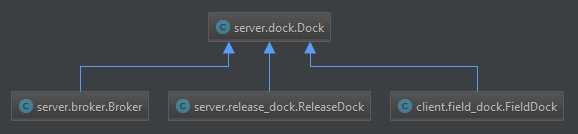
\includegraphics[scale=0.7]{afbeelding/classDock.png}}
\caption{Klassendiagram van Dock}
\label{fig:classDock}
\end{figure}

\paragraph{Grafische User Interfaces}
Het is ook mogelijk om de Grafische User Interface (GUI) op te starten door middel van de ``Enter'' toets.
Vanuit de GUI is het mogelijk om de verschillende clients te controleren en is het mogelijk om nieuwe installers te creëren.
De GUI werd gemaakt met de Python bibliotheek wxPython\footnote{\url{https://wxpython.org/}} en met de hulp van wxFormBuilder\footnote{\url{https://github.com/wxFormBuilder/wxFormBuilder}} werd basis code gegenereerd.
De nodige methodes werden vervolgens overschreven in de module overview\_impl.
Via deze methode wordt een gelijkaardig resultaat behaald voor het maken van de GUI voor de installer creatie.

\paragraph{Berichten versturen}
Bij het versturen van een bericht moet eerst een object aangemaakt worden van de Message klasse.
Vervolgens wordt de inhoud toegevoegd aan het bericht en kan het verzonden worden naar de broker.
In de broker wordt gecontroleerd welk type bericht het is om het dan vervolgens door te sturen naar alle doelen die in de gepaste list zitten.
Voordat het bericht wordt doorgestuurd wordt het eerst ingepakt in een ander bericht met als type notificatie.
Zo weet de ontvanger dat het bericht afkomstig is van de broker en is weet de ontvanger dat het data veld het doorgestuurde bericht bevat.
Deze kan vervolgens uitgepakt worden.
Afhankelijk van het type van het doorgestuurde bericht zal de correcte methode opgeroepen worden.

\paragraph{Installer creatie}
In de overzicht GUI is het mogelijk om een nieuwe installer te maken.
Met behulp van de aparte GUI, die geïmplementeerd wordt door de module release\_creator\_impl, is het mogelijk om een installer te definiëren.
Tijdens het samenstellen van de installer kunnen verscheidene nieuwe pakketten aangemaakt worden door de bovenste velden meermaals in te vullen.
Hierbij is het belangrijk om te weten dat een folder moet geselecteerd worden als bestandslocatie.
Alle bestanden aanwezig in de geselecteerde folder worden tijdens de creatie verplaatst naar de correcte locatie.
Bij het invullen van de gegevens van de installer moet ook een folder geselecteerd worden waarin de installer moet terecht komen.

Bij het indienen van de gegevens van de installer zelf worden de nodige handelingen uitgevoerd om een correcte installer te produceren.
Eerst worden de pakketten en installer toegevoegd aan de databank.
Vervolgens wordt de nodige folder structuur opgebouwd zoals aangegeven werd in Figuur~\vref{fig:installerStructuur}.
In de config folder wordt een leeg Dockerfile en een metadata bestand met daarin de volledige beschrijving van de installer.
Tijdens het creëren van de installer moet één van de pakketten aangeduid worden als een framework pakket.
Bij het toevoegen van de verschillende bestanden zal dit pakket een start\_script meekrijgen.
Dit is het script dat wordt uitgevoerd iedere keer als het framework wordt opgestart.
Hierna worden alle pakketten overlopen.
Als het pakket nieuw is, worden de nodige folders en bestanden aangemaakt anders worden de oude bestanden uit de meta folder gekopieerd.
Nadat de folder structuur aangemaakt is, is het mogelijk om de verschillende scripts aan te passen.
Net als bij het QT Installer Framework is het de bedoeling om te scripts te personaliseren naargelang het pakket.
Op deze wijze heeft ieder pakket een uniek installatie en test proces.
De installer is hierna klaar om gereleased te worden.
Van zodra in de overview GUI het release signaal gegeven wordt, schiet het tweede deel van het release proces in werking.
Een install agent wordt aangemaakt en wordt toegevoegd aan de lijst van agenten horende bij de installer.
De folder structuur uit het eerste deel wordt gezipt zodanig dat minder data verzonden moet worden.
Als laatste deel van wordt een ``release'' bericht aangemaakt en verzonden naar de broker.
Deze schiet vervolgens in gang en stuurt het bericht door naar de nodige field docks.

\paragraph{Client monitoring}
In de applicatie is het mogelijk om in een beperkte manier de clients te controleren.
De overview GUI bevat een tabel met de verschillende clients die aanwezig zijn in de databank.
Met hulp van de mysql.connector module van Python lukt het om de databank te ondervragen.
Alle gegevens over de torens wordt opgevraagd en vervolgens worden er Tower objecten van gemaakt.
Hierna wordt gecontroleerd of op de toren een installer aanwezig is.
Mocht dit zo zijn, worden de gegevens over deze installer uit de databank gehaald.
Op deze manier kan nagekeken worden welke installer aanwezig is en kan dit worden weergegeven in de GUI.

\section{Client-side}
\paragraph{Initialisatie}
Aan de client-side wordt een gelijkaardige werkwijze gebruikt als bij de server-side.
De module deployment\_client zal een field dock object aanmaken en de nodige services aanpassen.
Tijdens het eerste gebruik van de code wordt een controle uitgevoerd waarmee gecontroleerd wordt of de description\_file aanwezig is.
Dit bestand bevat de volledige beschrijving van de testtoren met alle verschillende hardware componenten.
Vervolgens gaat het field dock zich subscriben voor de nodige berichten bij de broker.
Als beide stappen zijn afgelopen, wordt de Grafische User Interface opgestart en is het systeem klaar om gebruikt te worden.

\paragraph{Eerste gebruik}
Bij het eerste gebruik van de applicatie is de description\_file nog niet aanwezig.
Er is dan nog geen beschrijving van de gebruiker aanwezig aan zowel de client- als server-side.
Om dit aan te pakken, wordt een GUI opgestart waarmee het mogelijk is om het volledige systeem te beschrijven.
Na het invullen van de nodige informatie en het indienen van alle gegevens, wordt de description\_file aangemaakt.
Een ``new'' bericht wordt gefabriceerd met in het data veld de volledige beschrijving van het systeem.
Dit bericht wordt verzonden naar de broker en de broker stuurt het bericht door naar iedereen die gesubscribed is voor de ``new'' berichten.
Het bericht komt toe bij het release dock.
Het bericht wordt uitgepakt, omgevormd naar een Tower object en vervolgens toegevoegd aan de databank.

\paragraph{Installatieproces}
Van zodra een ``release'' bericht binnen komt bij het field dock schiet deze in gang om het installatieproces op poten te zetten.
Met de informatie uit het bericht is het field dock in staat om een Installer object te maken.
Het field dock achterhaalt wie de zender van het bericht en contacteert dan direct de zender\footnote{Dit is het enige moment dat directe communicatie tussen de field en release docks mogelijk is}.
Nadat een connectie tussen de twee werd opgestart, wordt de gezipte installer samen met de nodige agenten verzonden naar het field.
Dill\footnote{\url{https://pypi.python.org/pypi/dill}} wordt gebruikt om de agent objecten te serialiseren voor ze verzonden worden naar het field dock.
De lijst van agenten wordt overlopen en het install agent object zal zijn functie uitvoeren.

De eerste actie die de install agent gaat ondernemen is het uitpakken van het zip bestand.
Met de Dockerfile uit de installer en de docker-py\footnote{\url{https://docker-py.readthedocs.io/en/stable/}} module wordt een Docker image aangemaakt die de basis zal vormen voor de container.
Voor de presentatie werd een image aangemaakt voor een Linux container waarin Python en wxPython op voorhand waren geïnstalleerd.
Vervolgens wordt een container gecreëerd met als naam ``fieldcontainer''.
Dit is de hoofdcontainer die altijd de laatst werkende versie van het framework zal bevatten.
Tijdens de creatie werden de nodige parameters doorgegeven om Grafische User Interfaces van de container op te kunnen starten.
Om dit mogelijk te maken, is het nodig om aan X11 forwarding te doen.
Belangrijk hierbij is dat op de host computer een X11 server moet draaien voordat dit kan plaats vinden.
Voor de demonstratie werd Cygwin\footnote{\url{https://www.cygwin.com/}} gebruikt om de X11 server op te starten en de correcte omgeving te generen\footnote{De tutorial \url{https://manomarks.net/2015/12/03/docker-gui-windows.html} werd hiervoor gevolgd}.
Hierna wordt het metadata bestand gelezen en gebruikt om de installatievolgorde van de pakketten te achterhalen.
Elk pakket wordt in de container gekopieerd en het installatie script wordt uitgevoerd.
Vervolgens gaat, met hulp van het test script, nagegaan worden of het installatieproces correct verlopen is.
De output van het script wordt gecontroleerd.
Als de uitgangsstatus begint met 0 wordt de test gezien als geslaagd.
Van zodra dit niet het geval is, wordt de container gemerkt als slecht en zal deze op het einde van het installatieproces in quarantaine geplaatst worden.
De container wordt niet verwijdert. 
Er werd voor deze strategie gekozen aangezien het mogelijk dat het test script slecht geschreven is.
Het framework is dan correct geïnstalleerd maar wordt door de test toch gezien als foutief.
Door de container in quarantaine te plaatsen blijft het mogelijk om achteraf test uit te voeren.
Vervolgens wordt een rapport aangemaakt met daarin het resultaat van de test, de begin- en eindtijd.
Het rapport wordt toegevoegd aan een bericht en wordt verzonden naar de broker die het doorstuurt.

\paragraph{Framework opstarten}
Na het opstarten van alle services verschijnt de Grafische User Interface van de client.
Van hieruit is het mogelijk om het pakket dat gemarkeerd staat als framework te openen.
De ``fieldcontainer'' wordt opgestart en het start script wordt uitgevoerd waardoor het framework zal opstarten.